\section{Fremgangsmetode}
Der skal udvikles en BMS uden en færdig kreds til styring og servicering af de centrale funktioner. Temperaturmåleren er beskrevet i kapitel \ref{sec:temperatur}, og vil derfor ikke blive gennemgået i dette kapitel.

\section{Måling af cellespændinger} \label{sec:cell_voltage}
Systemet er til hver en tid nødt til at kende den samlede cellespænding, for at vide hvornår opladning er nødvendig - og derfor ikke tillade underafladning. Da systemet samtidig skal være i stand til at måle de individuelle cellespændinger under opladning, er det derfor smart, at sætte en spændingsmåler hen over hver celle. På den måde kan de enkelte celler måles og batteripakkens udgangsspænding kan fås ved addition af alle celler.
\\

Måling af cellespænding kan opnås ved brug af en differensforstærker, for at få spændingsforskellen mellem hver celle. Outputtet af forstærkeren kan efterfølgende sendes ind i microens ADC. Da en celle kan variere mellem $3.2\volt$ og $4.2\volt$, samtidig med at microen er forsynet med $3.3\volt$, skal differensforstærkeren dimensioneres derefter. I praksis kan dette løses ved at have en forstærkning på mindre end 1, for at få outputtet til at svinge til microens forsyningsspænding ved maksimal cellespænding. Differensforstærkeren kan ses på figur \ref{fig:cell_voltage}.
\\

\begin{figure}[h]
	\centering
	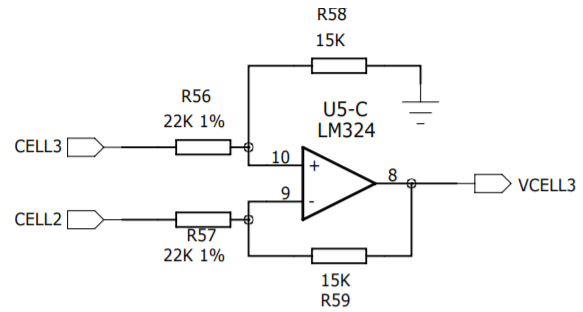
\includegraphics[width=11cm]{billeder/cell_voltage.png}
	\caption{Differensforstærker som spændingsmåler}
	\label{fig:cell_voltage}
\end{figure}

Operationsforstærkerens forstærkning udregnes,
\begin {equation} 
A_{v} = \frac{15\kilo\ohm}{22\kilo\ohm} = 0.68
\end {equation}

Udgangsspændingen på operationsforstærkeren er givet ved,

\begin {equation} 
V_{o} = V_{cell3} * \frac{R58}{R56+R58} * (1+\frac{R59}{R57}) - V_{cell2} * \frac{R59}{R57} \label{eq:op_amp_gain}
\end {equation}

Da en celle kan svinge mellem $3.2\volt$ og $4.15\volt$, vil microens ADC svinge mellem $2.176\volt$ og $2.822\volt$.

\section{Strømmåling}\label{afs:current_meas}
For at overvåge udgangsstrømmen skal en strømmåler realiseres. Dette kan gøres ved hjælp af en shunt modstand, $R_{s}$, som yder en meget lille og veldefineret ohmsk belastning og kan holde til hele udgangsstrømmen. Når belastningen trækker en strøm, vil et lille spændingsfald forekomme over shuntmodstanden, som en differensforstærker vil detektere og forstærke til et passende niveau. Der er i dette projekt valgt, at placere shuntmodstanden på lav-siden mellem den nedeste celle og aflade MOSFET'en.
\\

Da den maksimale aflade- og opladestrøm  er $I_{out} = 6\ampere$ og $I_{In} = 1\ampere$, skal microen kunne skelne mellem om den er igang med at blive opladt eller afladt, er en retningsbestemmelse på strømtrækket nødvendig.
\\

Der er i dette projekt undersøgt flere muligheder til detektering af strømmen. En af iterationerne var en enkelt differensforstærker til begge målinger, med at offsette spænding ved $0\volt$ til enten $1.65\volt$ eller $6\volt$ alt afhængig af forsyningsspændingen.
\\

For optimal anvendelse af microens opløsning er der i projektet valgt at opbygge to differensforstærkere, en for afladning og opladning. Både strømåling til op- og afladning sker hen over den samme shuntmodstand og kan ses på figur \ref{fig:current_sense}.

\begin{figure}[h]
	\centering
	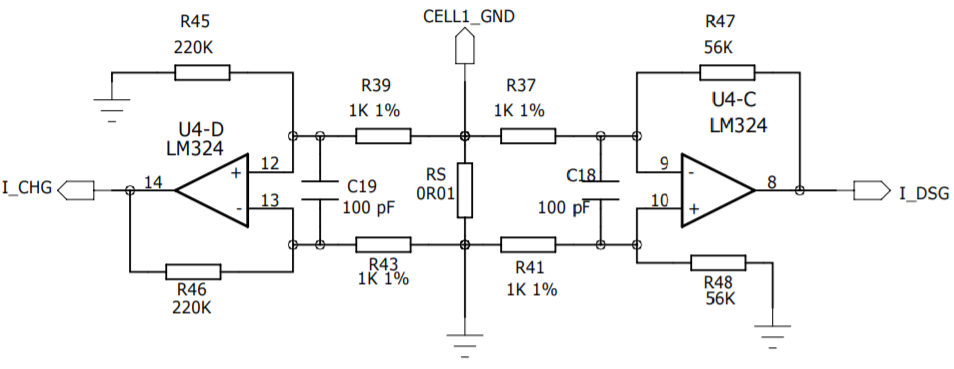
\includegraphics[width=15cm]{billeder/current_meassurement.png}
	\caption{Differensforstærkere som strømmåler}
	\label{fig:current_sense}
\end{figure}

En vigtig parameter under dimensionering af en strømmåler er valg af shunt modstandens værdi. Ud fra den maksimale afladestrøm $I_{out} = 6\ampere$ vælges shunt modstanden $R_{s} = 10\milli\ohm$. Det maksimale spændingsfald $V_{s}$ over shuntmodstanden bliver,

\begin {equation} 
V_{s} = I_{out} * R_{s}  = -6\ampere * 10\milli\ohm = -60\milli\volt
\end {equation}

Spændingsfaldet vil ligge mellem $0\milli\volt$ og $-60\milli\volt$ (grundet strømmens retning). 
Da microcontrolleren kører med en logik på $3.3\volt$ og har en ADC med en opløsning på 12 Bit, skal signalet dimensioneres efter dette. Med en shuntmodstand på $10\milli\ohm$ vil den under opladning have et spændingsfald på $10\milli\volt$, og derfor, grundet retningsskift af strømmen, skal strømmåleren tage hensyn til dette.
\\

For valg af shuntmodstand skal der tages højde for den maksimale effektafsættelse i den og udregnes $60\milli\volt * 6\ampere = 360\milli\watt$. Den valgte shuntmodstand kan klare $3\watt$.
\\

Ved hjælp af en to differensforstærkere kan et brugbart indgangssignal til ADC'en realiseres for både opladning og afladning. Forstærkerne er opbygget med en operationsforstærkere koblet med negativ feedback.
\\

Den maksimale forstærkning $A_{v}$ af signalet for måling af afladestrømmen findes,
\begin {equation} 
A_{v} = \frac{V_{o}}{V_{s}} = \frac{3.3\volt}{60\milli\volt} = 55
\end {equation}

For at opnå denne forstærkning anvendes en indgangsmodstand ($R37$) på $1\kilo\ohm$ og en $47\kilo\ohm$ modstand på feedbacken ($R47$), for at blive på $E6$-serien. Udgangsspændingen fås ved brug af ligning \ref{eq:op_amp_gain}, hvor $V_{cell3} = V+$ og $V_{cell2} = V+$. For at overskueliggøre beregningen vælges $R41 = R37$ og $R47 = R48$. Med disse modstandsværdier fås en forstærkning på $A_{v} = 47$
\\

Som tidligere nævnt vil et retningsskifte af strømmen forekomme under opladning, så forstærkeren skal kunne trigge på et positivt spændingsfald. Ved at vende operationsforstærkeren om, kan måling af strømmen ved opladning ske uden brug af en negativ forsyning.
\\

Da opladestrømmen er $1\ampere$ kan en væsentlig højere forstærkning anvendes, hvilket giver en højere præcision på ADC'en. Ved brug af samme formel som den anden differensforstærker, beregnes $V_{o}$ for måling af opladestrøm. $R39 = R49 = 1\kilo\ohm$ og $R45 = R469 = 220\kilo\ohm$ og giver en forstærkning på 20 gange. Spændingen vil derfor variere mellem $0\volt$ og $2.2\volt$. I tilfælde af at en højere opladningsstrøm ønskes, er forstærkningen ikke højere, for stadig at kunne måle strømmen.


\section{Passiv balancering}\label{afs:balancing}

Når batteripakkens opladecyklus er ved at være færdig og den første celle er fuldt opladt, vil passiv balancering blive aktiveret. Batteripakken vil maksimalt balancere tre celler på en gang, da den er færdig med at oplade når den får signal om, at alle fire celle har behov for balancering, da de jo har nået den maksimale cellespænding.
\\

Balanceringskredsen kan ses på figur \ref{fig:passiv_balancering} består af tre modstande, en PNP ($Q5$) og NPN ($Q6$) transistor. $R21$ er afladningsmodstanden, som under balancering vil yde en belastning på cellen og aflade den til samme spænding som den laveste opladte celle. $R19$ ligger et arbejdspunkt på basen af $Q5$ og $R20$ begrænser strømmen til microcontrolleren. 
\\

\begin{figure}[h]
	\centering
	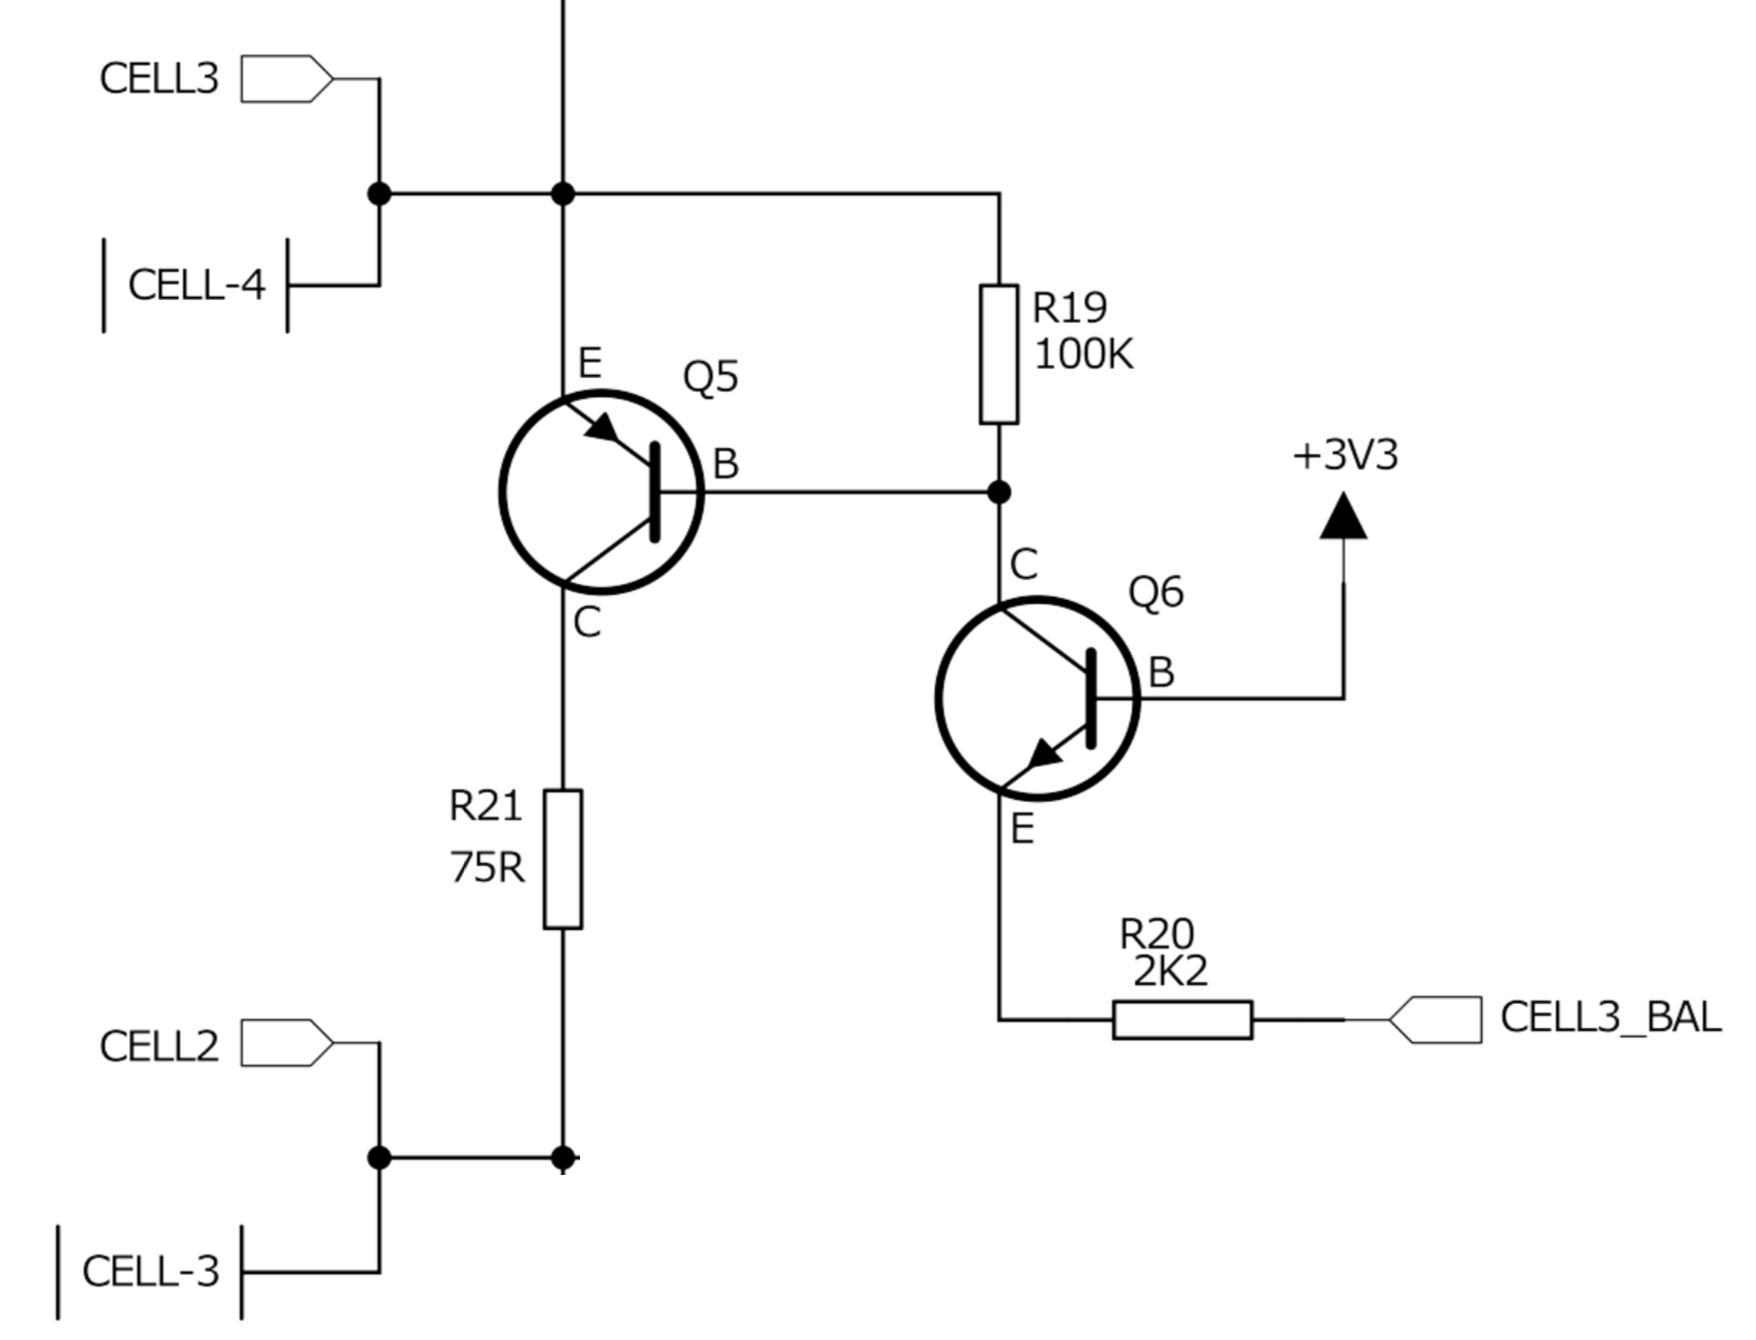
\includegraphics[width=10cm]{billeder/balance.png}
	\caption{Passiv balancering af celler under opladning}
	\label{fig:passiv_balancering}
\end{figure}

Basen på $Q6$ er forspændt med $3.3\volt$ og under afladning vil microcontrolleren sætte benet højt på emitteren, hvilket holder $Q6$ slukket. For at aktivere balancering, skal potentialet på basen af $Q5$ være en base-emitter strækning lavere end dens emitter. Dette kan gøre ved at sætte microcollerens ben lav, hvilket vil tænde $Q6$, trække potentialet på basen af $Q6$ ned og derved lede strømmen igennem $R21$. $R21$ består af to 0805-$150\ohm$ modstande for at få en modstandsværdi på $75\ohm$ som kan klare $2 x 125\milli\watt = 250\milli\watt$. Med denne modstand vil balanceringsstrømmen maksimalt blive $50\milli\ampere$ og have en effektafsættelse på $190\milli\watt$.

\section{MOSFET driverkreds}
Batteripakken skal kunne afbrydes fra en belastning i tilfælde af fejlsituationer. For at kunne opnå dette, er to MOSFET'er i en fælles drain konfiguration valgt og virker som en to tovejs kontakt. De kan både være placeret på $V_{pack+}$ og $V_{pack-}$. Hvis en N-kanal MOSFET er på $V_{pack+}$ skal gaten tændes med $V_{out} + V_{gs}$, hvilket i denne applikation giver en spænding på $V_{gs} = 28.8\volt$. For at kunne opnå denne spænding vil en charge pumpe være nødvendig. For at undgå brug af en charge pumpe kan en P-kanal MOSFET anvendes. Udvalget på P-kanal MOSFET'er er dog begrænset og de har en væsentlig højere ledemodstand, $R_{DS-ON}$. 
\\

En anden mulig placering af MOSFET'erne er på $V_{pack-}$. Fordelen ved denne placering er, at de skal tændes i forhold til stel. Ulempen er at stelplanet kan påvirkes negativt, når blandt andet batteripakkens nederste celle ikke er forbundet direkte til stelplanet.
\\

I dette projekt vælges der at MOSFET'erne placeres på $V_{pack-}$, for nemmere at kunne tænde dem. Aflade-MOSFET'en skal altid tændes i forhold til stel, hvorimod et problem kan opstå ved oplade-MOSFET'en, hvor den ikke kan tændes. Det drejer sig om en fejlsituation hvor de begge er slukkede, men en belastning er koblet på. Spændingen på oplade-MOSFET'ens source kan derfor drive op til terminalspænding gennem belastningen og kan derfor ikke tændes før den anden MOSFET er tændt, da den skal trække potentialet ned igen. Når den anden MOSFET skal trække potentialet ned, kan det kun ske igennem oplade-MOSFET'ens bodydiode, hvilket med et spændingsfald på omkring $1\volt$ og et maksimalt strømtræk på $6\ampere$ medfører en kortvarig effektafsættelse i MOSFET'en på $6\watt$. En måde at omgå dette problem er ved brug af en P-kanal MOSFET som kan ses i afsnit \ref{afs:bms_ic_desc}.


\begin{figure}[h]
	\centering
	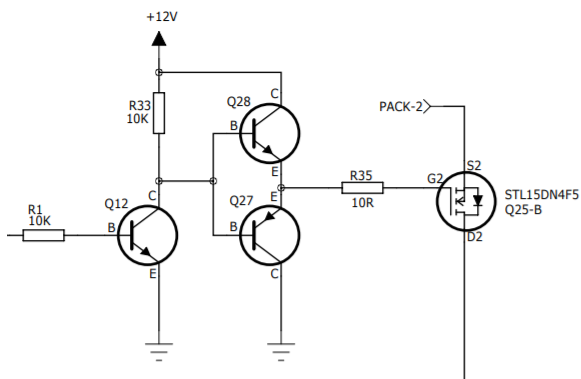
\includegraphics[width=10.5cm]{billeder/mosfet_driver.png}
	\caption{MOSFET driverkreds}
	\label{fig:mosfet_driver}
\end{figure}

Driveren til begge MOSFET'er er ens og kan ses på figur \ref{fig:mosfet_driver}. Driveren består af en NPN ($Q28$) og PNP ($Q27$) BJT koblet i en push-pull konfiguration. For at kunne tænde og slukke driveren gøres der brug af en NPN BJT. Gate modstanden $R35$ er valgt til $10\ohm$ for hurtig styring af MOSFET'en. De to MOSFET'er er altid tændte, og slukker kun i tilfælde af fejlsituationer.

\section{Sikkerhed ved overstrøm}
For at beskytte batteripakken ved en overstrøm under op- eller afladning, skal sikkerhedsforanstaltninger realiseres. Igennem dette projekt har flere iterationer været nødvendige, før den endelige løsning kom på plads. Problemet med tidligere versioner var, at i tilfælde af for store strømtræk af en belastning, ville systemet sagtens kunne registrere dette og efterfølgende slukke for MOSFET'erne. Problemet opstod dog efterfølgende når belastningen stadig var koblet til. Efter detektering af en overstrøm ville en ny strømmåling blive foretaget, her hvor pakken nu var afbrudt. Den ville så opdage, at forholdene var optimale til at køre igen, så MOSFET'erne ville tænde, men en ny måling ville så igen detektere en overstrøm. Her ville den så ende med at oscillere mellem de to tilstande. 
En overstrømsdetektor der kan holde sig slukket ved tilfælde af for store strømtræk under op- og afladning var nødvendig. Det vil derfor blive microcontrollerens opgave at tillade en forbindelse mellem batteripakke og belastning.
\\

Formålet med at have dedikeret hardware til at trigge på overstrøm i stedet for lade det hele blive styret af microcontrolleren er, at den dedikerede hardware har væsentlig hurtigere reaktionshastighed end micro'en. Når micro'en detekterer en overstrøm har dedikerede hardware allerede slukket for MOSFET'erne og dermed undgået forøget risici for beskadigelse af batteripakken.
\\

\subsection{Overstrøm ved afladning}\label{sec:overcurrent_dsg}
For at kunne detektere for stort strømtræk under afladning, skal information omkring strømstørrelsen bruges som reference. Spændingsfaldet hen over shuntmodstanden bliver i denne konstruktion anvendt til at afbryde batteripakken fra belastningen.
\\

Figur \ref{fig:overcurrent_discharge} viser måden hvorpå beskyttelsen er realiseret i dette projekt. Nettet $CELL1GND$ er forbundet med den nederste celles GND-terminal, shuntmodstanden og beskyttelse for både op- og afladning. Under drift vil spændingen kunne variere mellem $-60\milli\volt$ og $10\milli\volt$, da strømmens retning kan variere alt afhængig af hvad der kobles til udgangsterminalerne. Under afladning vil spændingen dog kun kunne variere mellem $0\volt$ og $-60\milli\volt$ ved $6\ampere$.
\\

\begin{figure}[h]
	\centering
	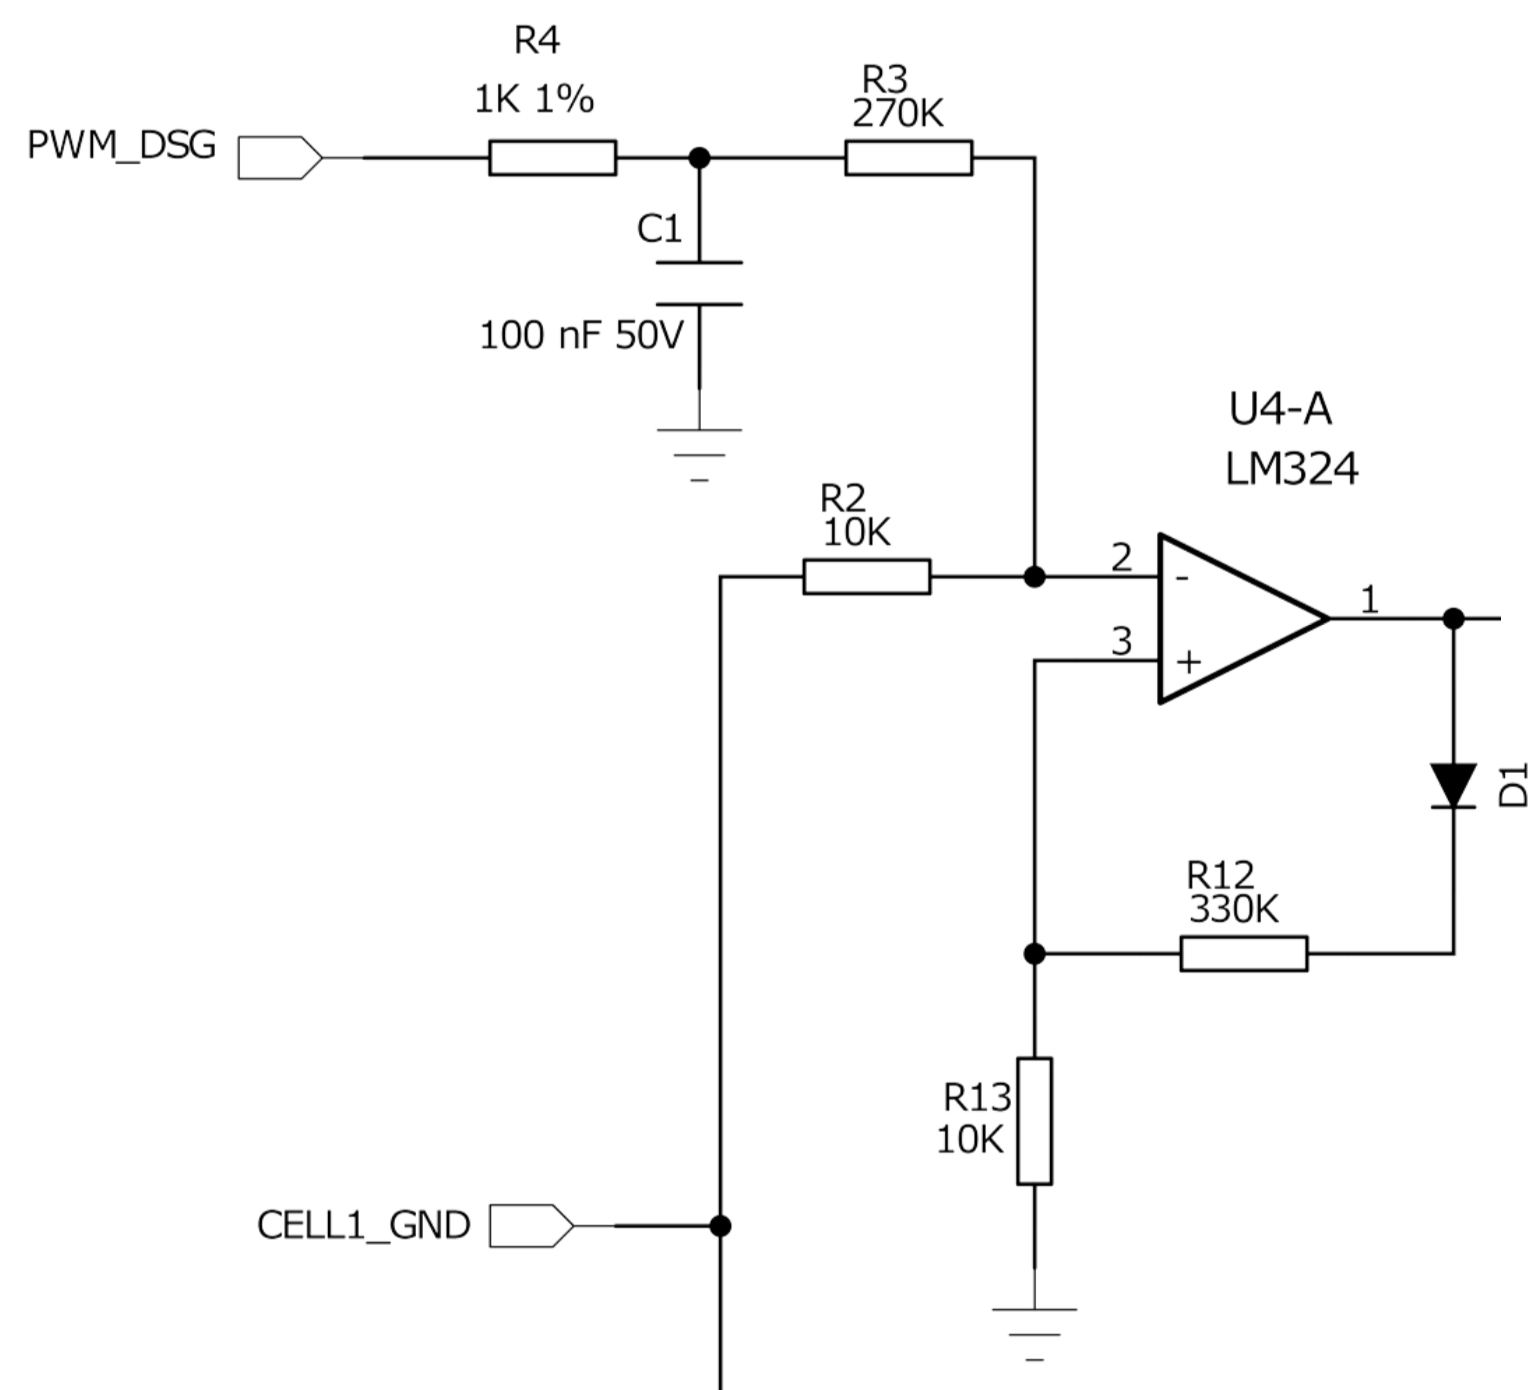
\includegraphics[width=11cm]{billeder/overcurrent_discharge.png}
	\caption{Sikkerhed for overstrøm under afladning}
	\label{fig:overcurrent_discharge}
\end{figure}

$PWM-DSG$ går til et ben på microcontrolleren. Benet generer et PWM signal og bliver glattet ud af kondensatoren $C1$, så spændingen bliver $1.7\volt$. PWM signalet styrer i denne konfiguration hvor stor en afladningsstrøm der tillades fra batteripakken. $R3$ og $R2$ spændingsdeler PWM signalet,

\begin {equation} 
V_{DSG} = V_{PWM-DSG} * \frac{R_{2}}{R_{3}+R_{2}} = 1.7\volt * \frac{10\kilo\ohm}{270\kilo\ohm + 10\kilo\ohm} = 60.7\milli\volt
\end {equation}

Når der ikke er noget koblet på udgangsterminalerne, vil der ligge $60\milli\volt$ på operationsforstærkerens inverterende indgang, og outputtet fra operationsforstærkeren er $0\volt$. 

Outputtet er forbundet gennem $10\kilo\ohm$ til basen på $Q12$ der kan tænde og slukke for MOSFET driveren til $Q25-B$.
\\

Aflades batteripakken inden for specifikationerne, $0\ampere$ til $6\ampere$, vil spændingen på operationsforstærkerens inverterende indgang variere i knudepunktet ud fra bidraget,

\begin {equation} 
V_{-} = V_{PWM-DSG} + V_{CELL1-GND} = 60\milli\volt + V_{PWM-DSG}
\end {equation}

Under afladning antager $V_{PWM-DSG}$ negativ værdi. Når bidraget fra  strømtrækket overstiger grænsen, vil potentialet på $V-$ blive negativ og dermed blive lavere end $V+$, som vil få operationsforstærkerens udgang til at gå høj. Da den er forsynet med $3.3\volt$ vil den udgangen ideelt set antage samme potentiale. Som tidligere nævnt er operationsforstærkerens udgang forbundet med basen på $Q12$ som dermed tændes og slukker driveren.
\\

Samtidig med at driveren slukkes leder dioden $D1$ og forspænder $V+$ gennem en spændingsdeling af $R12$ og $R13$. Schottky diodernes opgave i både op- og afladning er dertil at levere et spændingsfald på $0.3\volt$, for at sikre at kredsen kan nulstilles. Potentialet på $V+$ vil efter en overstrøms situation være,

\begin {equation} 
V_{+} = (V_{High} - V_{diode} ) * \frac{R_{13}}{R_{12}+R_{13}} = (3.3\volt - 0.3\volt ) * \frac{10\kilo\ohm}{330\kilo\ohm + 10\kilo\ohm} =  88\milli\volt
\end {equation}

Når kredsen har trigget og slukket driveren, vil MOSFET'en, $Q25_B$, forblive slukket selvom belastningen kan være frakoblet. Når MOSFET'en er slukket vil den ikke lede og bodydioden vil blokere strømmen.
Hvis intet er koblet på udgangsterminalerne eller en belastning der trækker under $6\ampere$ er tilkoblet vil potentialet på $V-$ være positiv og maksimalt $60\milli\volt$. Operationsforstærkeren vil forblive høj på udgangen da,

\begin {equation} 
V+ > V- \quad = \quad 88\milli\volt > 60\milli\volt
\end {equation}

På den måde har operationsforstærkeren en indbygget hysterese.
Microcontrolleren vil opdage en overstrøms situation, men behøver ikke at slukke driveren, da det allerede sker før den opdager dette. For at tænde MOSFET'en skal operationsforstærkerens "hysterese" \space nulstilles, og dette gøres ved, at sende en puls på $3.3\volt$ fra $PWM_DSG$, hvilket får $V-$ til at komme op på $117.9\milli\volt$, og dermed overstiger $V+$.


\subsection{Overstrøm ved opladning}\label{sec:overcurrent_chg}
For at beskytte batteripakken mod for stor strøm under opladning, skal der ligesom afladningsbeskyttelse udvikles noget dedikeret elektronik der reagerer hurtigere en microcontrolleren. Den færdige kreds kan ses på figur \ref{fig:overcurrent_charge}. Den maksimale opladestrøm er i kravspecifikationen $I_{In}=1\ampere$, men vil i realiteten blive $1.07\ampere$, hvilket stadig er acceptabelt da cellerne i projektet er godkendt til opladning med 1C ($2600\milli\ampere$).
\\

\begin{figure}[h]
	\centering
	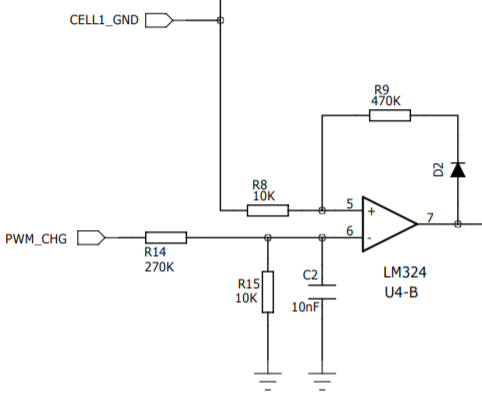
\includegraphics[width=11cm]{billeder/overcurrent_charge.png}
	\caption{Sikkerhed for overstrøm under opladning}
	\label{fig:overcurrent_charge}
\end{figure}

Nettet $PWM-CHG$ genererer en spænding gennem PWM på $300\milli\volt$ hvilket gennem spændingsdeling af $R14$ og $R15$ ligger et $10.7\milli\volt$ potentiale på $V-$. Under afladning kan nettet $CELL1_GND$ svinge mellem $0\volt$ og op til $10.7\milli\volt$. Hvis spændingen kommer over $V-$, går operationsforstærkeren høj, hvilket slukker for $Q13$. Gennem dioden og spændingsdelingen mellem $R9$ og $R8$, vil potentialet på $V+$ forblive $58.3\milli\volt$.
\\

For at resette operationsforstærkerens hysterese sendes en puls fra $PWM-CHG$ på $3.3\volt$ igennem spændingsdeleren, så spændingen på $V-$ bliver $117.9\milli\volt$.


\section{Spændingsnet}\label{afs:voltagenet}
Forsyningsspændingen til hele BMS'en kommer fra batteripakkens terminalspænding, som kan variere mellem $12.8\volt - 16.6\volt$. For at generere to nødvendige netspændinger på $12\volt$ og $3.3\volt$, skal to spændingsregulatorer realiseres.
\\

Til at nedtrappe spændingen fra terminalspænding som maksimalt kan være $16.8\volt$ ned til $12\volt$ er en N-kanal zener spændingsregulator valgt. MOSFET'en der anvendes er 2N7002 og er godkendt op til $60\volt$. Valget af netop denne MOSFET er også grundet dens lave threshold spænding $V_{GS(th)}$ på omkring  $1.5\volt$.
\\


Udgangen af $12\volt$-spændingsregulatoren er MOSFET'ens source. For at finde zener diodens zener-spænding anvendes følgende formel,

\begin {equation} 
V_{z} = V_{o} + V_{GS(th)} = 13.5\volt
\end {equation}

For at nedtrappe spændingen fra $12\volt$ til $3.3\volt$ anvendes LDO'en TS9011SCX. Den har en absolut maksimum indgangsspænding på $12\volt$, hvilket medfører at zenerdioden vælges til $V_{z}=12\volt$. Med denne værdi bliver $12\volt$-nettet nærmere $10.5\volt$, hvilket i dette projekt er acceptabelt - nettet kaldes dog fortsat $12\volt$-nettet.
\\

Kredsløbet kan ses på figur \ref{fig:voltage_nets}, og virker på den måde, at zener dioden trækker strøm gennem $R10$, så spændingen på MOSFET'ens gate bliver diodens zener-spænding. Når MOSFET'ens gate-source spænding $V_{GS(th)}$ rammer sit arbejdspunkt, vil MOSFET'en fungere som en variabel modstand, og have et spændingsfald over drain-source så den stadig kan holde gaten tændt. For at minimere strømforbruget i batteripakken er $3.3\volt$ forsyningen valgt til at være TS9011SCX, da den er af typen "Low Quiescent Current CMOS", og kun bruger $2\micro\ampere$ til at regulere udgangspændingen.

\begin{figure}[h]
	\centering
	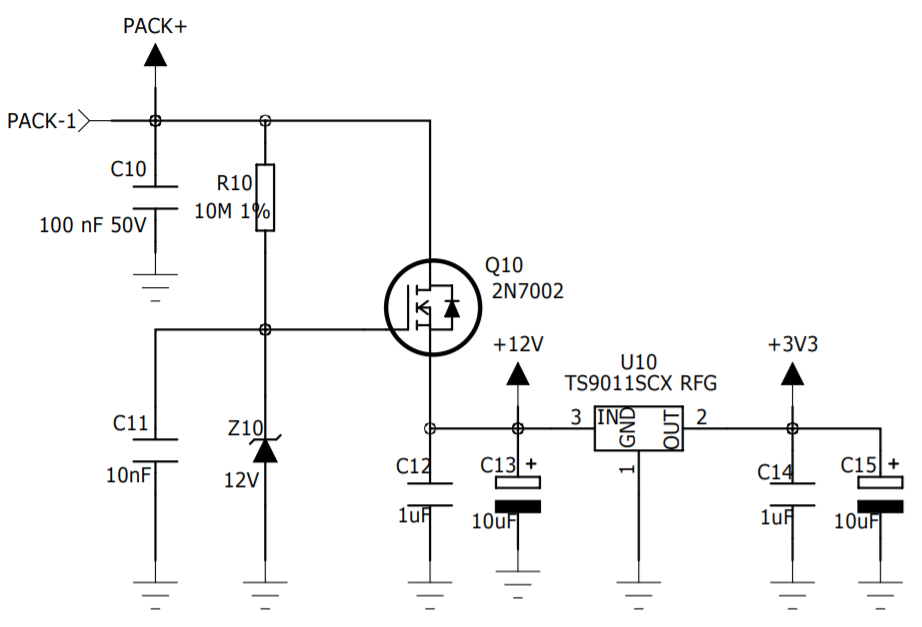
\includegraphics[width=12cm]{billeder/voltage_nets.png}
	\caption{Generering af 3.3V og 12V}
	\label{fig:voltage_nets}
\end{figure}

\section{Standby tilstand}
En standby tilstand kan både indeholde tiltag i hardwaren og softwaren.

\subsection{Hardware}
I den diskret udviklede batteripakke, indgår der ikke nogle tiltag hvori en standby tilstand kan opnås. Der er blevet undersøgt forskellige muligheder såsom at forsyne operationsforstærkerne fra microcontrolleren til måling af cellespænding og strømtræk. Disse tiltag er dog ikke blevet realiseret da batteripakken som standard tilstand altid tillader op- og afladning, så hvis batteripakken skal kunne detektere noget på udgangen, skal operationsforstærkerne også være tændte.

\subsection{Software}
Microcontrolleren har flere stadier af power-down modes, men siden PWM output ikke er tilgængeligt under disse modes, og da PWM bliver brugt til at styre MOSFET's til op- og afladningskontrol, er det blevet fravalgt at implementere dette. 

\section{Delkonklusion}
Igennem udviklingen af batteripakken uden brug af en integreret styringskreds, er alle funktionaliteter blevet realiseret. Batteripakken at aflades med $6\ampere$ og oplades med $1\ampere$. Der er ikke udviklet en buck converter til at begrænse opladestrømmen, så for at oplade batteripakken, skal opladeren stå for strømbegrænsningen.
\\

Batteripakken kan til hver en tid lave målinger på cellespænding og strømtræk, hvor den også kan detektere om en belastning eller oplader er koblet på udgangen. Der er derudover også realiseret en løsning til passiv balancering.